% !TeX spellcheck = pt-BR
\documentclass[
	% -- opções da classe memoir --
	12pt,				% tamanho da fonte
%	openright,			% capítulos começam em pág ímpar (insere página vazia caso preciso)
	oneside,			% para impressão em recto e verso. Oposto a oneside
	a4paper,			% tamanho do papel. 
	% -- opções da classe abntex2 --
	%chapter=TITLE,		% títulos de capítulos convertidos em letras maiúsculas
	%section=TITLE,		% títulos de seções convertidos em letras maiúsculas
	%subsection=TITLE,	% títulos de subseções convertidos em letras maiúsculas
	%subsubsection=TITLE,% títulos de subsubseções convertidos em letras maiúsculas
	% -- opções do pacote babel --
	english,			% idioma adicional para hifenização
	french,				% idioma adicional para hifenização
	spanish,			% idioma adicional para hifenização
	brazil,				% o último idioma é o principal do documento
	%article,
	]{abntex2}


% ---
% PACOTES
% ---

% ---
% Pacotes fundamentais 
% ---
\usepackage{lmodern}			% Usa a fonte Latin Modern
\usepackage[T1]{fontenc}		% Selecao de codigos de fonte.
\usepackage[utf8]{inputenc}		% Codificacao do documento (conversão automática dos acentos)
\usepackage{indentfirst}		% Indenta o primeiro parágrafo de cada seção.
\usepackage{color}				% Controle das cores
\usepackage{graphicx}			% Inclusão de gráficos
\usepackage{microtype} 			% para melhorias de justificação
\usepackage{float}
% ---

% ---
% Pacotes adicionais, usados no anexo do modelo de folha de identificação
% ---
\usepackage{multicol}
\usepackage{multirow}
% ---
	
% ---
% Pacotes adicionais, usados apenas no âmbito do Modelo Canônico do abnteX2
% ---
\usepackage{amsmath}
\usepackage{graphicx}
\graphicspath{ {images/} }
\usepackage[colorinlistoftodos]{todonotes}

% not from template
\usepackage{lipsum}
%\usepackage{tikz}
\usepackage{pgfplots}
\usetikzlibrary{shapes,shapes.geometric,arrows,fit,calc,positioning,automata,patterns,matrix,arrows.meta, shapes.geometric, arrows,chains}

\usepackage{verbatim}
\usepackage{blindtext}
\usepackage{enumitem}
\usepackage{multicol}
\usepackage{listings}
\newcommand*{\euler}{\mathrm{e}}

\usepackage{fancyvrb}
\usepackage{hyperref}
\usepackage{relsize}

\usepackage{caption}
\usepackage{subcaption}
\usepackage{multicol}
% ---

% ---
% Pacotes de citações
% ---
\usepackage[brazilian,hyperpageref]{backref}	 % Paginas com as citações na bibl
\usepackage[alf]{abntex2cite}	% Citações padrão ABNT

% --- 
% CONFIGURAÇÕES DE PACOTES
% --- 

% ---
% Configurações do pacote backref
% Usado sem a opção hyperpageref de backref
%\renewcommand{\backrefpagesname}{Citado na(s) página(s):~}
\renewcommand{\backrefpagesname}{}
% Texto padrão antes do número das páginas
\renewcommand{\backref}{}
% Define os textos da citação
\renewcommand*{\backrefalt}[4]{
	\ifcase #1 %
		Nenhuma citação no texto.%
	\or
		Citado na página #2.%
	\else
		Citado #1 vezes nas páginas #2.%
	\fi}%
% ---

%%%% TIKZ HEADERS - Fabio

\tikzset{
	startstop/.style={
		rectangle, 
		rounded corners,
		minimum width=4cm, 
		minimum height=1cm,
		align=center, 
		draw=black, 
		fill=gray!70
	},
	startstop2/.style={
		rectangle, 
		rounded corners,
		minimum width=4cm, 
		minimum height=1cm,
		align=center, 
		draw=black, 
		fill=green!30
	},
	process/.style={
		rectangle, 
		minimum width=4cm, 
		minimum height=1cm, 
		align=center, 
		draw=black, 
		fill=gray!30
	},
	process2/.style={
		rectangle, 
		minimum width=4cm, 
		minimum height=1cm, 
		align=center, 
		draw=black, 
		fill=red!30
	},
	process3/.style={
		rectangle, 
		minimum width=4cm, 
		minimum height=1cm, 
		align=center, 
		draw=black, 
		fill=green!30
	},
	decision/.style={
		rectangle, 
		minimum width=4cm, 
		minimum height=1cm, align=center, 
		draw=black, 
		fill=green!30
	},
	arrow/.style={thick,->,>=stealth},
	dec/.style={
		ellipse, 
		align=center, 
		draw=black, 
		fill=black!30
	},
}

%%% end TIZK HEADERS - Fabio

% ---
% Informações de dados para CAPA e FOLHA DE ROSTO
% ---
\titulo{Atividade Final}
\autor{Bruno Canale \\ Bruno Giordano \\ Fábio T. Sancinetti \\ Wanderson Ferreira}
\local{São Paulo - Brasil}
\data{07 de dezembro de 2016}
\instituicao{%
  Universidade de São Paulo
  \par
  Escola Politécnica
  \par
  Programa de Pós-Graduação em Engenharia Elétrica \par PPGEE }
\tipotrabalho{Atividade Final}
% O preambulo deve conter o tipo do trabalho, o objetivo, 
% o nome da instituição e a área de concentração 
\preambulo{ \textbf{PSI5886} Princípios de Neurocomputação \break \textbf{Professor}: Emílio Del Moral Hernandez \break \break \textbf{Atividade Final}: Redes Neurais Convolucionais }
% ---

% ---
% Configurações de aparência do PDF final

% alterando o aspecto da cor azul
\definecolor{blue}{RGB}{41,5,195}

% informações do PDF
\makeatletter
\hypersetup{
		%pagebackref=true,
		pdftitle={\@title}, 
		pdfauthor={\@author},
		pdfsubject={\imprimirpreambulo},
		pdfcreator={},
		pdfkeywords={PSI5886}{Redes Neurais}{atv\_final}, 
		colorlinks=true,       		% false: boxed links; true: colored links
		linkcolor=black,          	% color of internal links
		citecolor=black,        	% color of links to bibliography
		filecolor=black,      		% color of file links
		urlcolor=black,
		bookmarksdepth=4
}
\makeatother
% --- 

% --- 
% Espaçamentos entre linhas e parágrafos 
% --- 

% O tamanho do parágrafo é dado por:
\setlength{\parindent}{1.3cm}

% Controle do espaçamento entre um parágrafo e outro:
\setlength{\parskip}{0.2cm}  % tente também \onelineskip

% ---
% compila o indice
% ---
\makeindex
% ---


% --- styles

\tikzstyle{input}=[draw,fill=white!50,circle,minimum size=20pt,inner sep=0pt]
\tikzstyle{hidden}=[draw,fill=white!50,circle,minimum size=20pt,inner sep=0pt]
\tikzstyle{output}=[draw,fill=white!50,circle,minimum size=20pt,inner sep=0pt]
\tikzstyle{bias}=[draw,dashed,fill=gray!50,circle,minimum size=20pt,inner sep=0pt]

\tikzstyle{stateTransition}=[->, thick]


\usepackage{afterpage}

% ----
% Início do documento
% ----
\begin{document}

% Seleciona o idioma do documento (conforme pacotes do babel)
%\selectlanguage{english}
\selectlanguage{brazil}

% Retira espaço extra obsoleto entre as frases.
\frenchspacing 

% ----------------------------------------------------------
% ELEMENTOS PRÉ-TEXTUAIS
% ----------------------------------------------------------
% \pretextual

% ---
% Capa
% ---
%\imprimircapa
% ---

% ---
% Folha de rosto
% (o * indica que haverá a ficha bibliográfica)
% ---
\imprimirfolhaderosto
% ---

% ---
% inserir lista de tabelas
% ---
%\pdfbookmark[0]{\listtablename}{lot}
%\listoftables*
%\cleardoublepage
% ---

% ---
% inserir lista de abreviaturas e siglas
% ---
\begin{siglas}
	\item[CNN] \textit{Convolutional Neural Networks} - Redes Neurais Convolucionais
	\item[GPU] \textit{Graphic Processor Unit} - Unidade de Processamento Gráfico
	\item[MLP] \textit{Multilayer Perceptron} - Perceptron em muti-camadas
	\item[RNA] Redes Neurais Artificiais
	\item[RNN] \textit{Recurrent Neural Networks} - Redes Neurais Recorrentes
\end{siglas}
% ---

% ---
% inserir lista de símbolos
% ---
%\begin{simbolos}
%  \item[$ \Gamma $] Letra grega Gama
%  \item[$ \Lambda $] Lambda
%  \item[$ \zeta $] Letra grega minúscula zeta
%  \item[$ \in $] Pertence
%\end{simbolos}
% ---

% ---
% inserir o sumario
% ---
\pdfbookmark[0]{\contentsname}{toc}
\tableofcontents*
%\cleardoublepage

% ---


% ----------------------------------------------------------
% ELEMENTOS TEXTUAIS
% ----------------------------------------------------------
\textual

% ----------------------------------------------------------
% Introdução (exemplo de capítulo sem numeração, mas presente no Sumário)
% ----------------------------------------------------------
\chapter[Introdução]{Introdução}

\par \lipsum[50]

\chapter{LIPSUM}
\section{Wolverinis Adamantium}
\par \lipsum[30] \cite{deeplearning_net_mlp}

\par Exemplo de citação em linha segundo \citeonline{rojas1996} aqui.

\chapter{Visualização do reconhecimento em uma Rede Neural}
\section{Base de dados: MNIST}

\par A base de dados MNIST (\textit{Mixed National Institute of Standards and Technology}) por \citeonline{mnistlecunn}, é uma base de dados que contem 60000 exemplos de digitos manuscritos para treino e outros 10000 exemplos para treino disponível em \url{http://yann.lecun.com/exdb/mnist/}.

\par As imagens dos dígitos possuem 28x28 pixels, entretanto os dígitos em si possuem 20x20, são normalizados e centralizados.

\begin{figure}
	\centering
	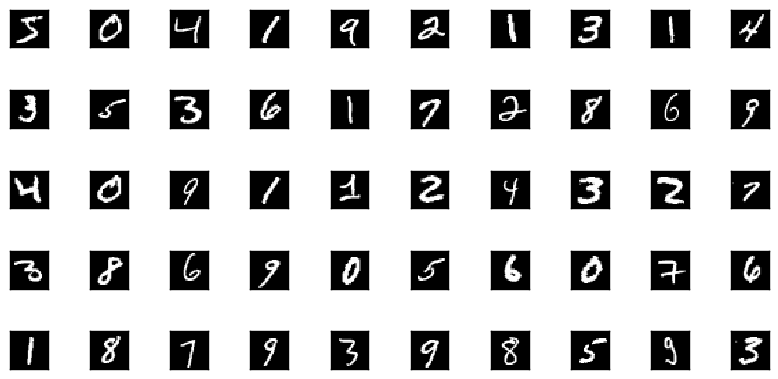
\includegraphics[width=0.7\linewidth]{images/fabio/inputs}
	\caption[Exemplos dos 50 primeiros digítos disponíveis na base de dados do MNIST.]{}
	\caption{}
	\label{fig:inputs}
\end{figure}

\par Segundo \citeonline{mnistlecunn}, algumas técnicas de reconhecimento de dígitos foram aplicadas a esses bancos como classificadores lineares, KNN (K-nearest neighbors), entre outras, obtendo taxa de erro entre 12\% e 0.54\% respectivamente. Entretanto, como o objetivo deste trabalho é auxiliar o entendimento dos funcionamento das redes convolucionais através da visualização dos resultados, os valores de taxa de erro mais interessantes são os relacionados a redes convolucionais similares as apresentadas nesse trabalho. \citeonline{mnistlecunn} apresenta redes convolucionais de LeNet-1, LeNet-4, LeNet-5 com taxas de erro de 1.7\%, 1.1\% e 0.7\% respectivamente. \citeonline{mnistlecunn} ainda apresenta os resultados para outras redes convolucionais com medida de erros como \textit{cross-entropy} com taxas de erro de 0.6\%,

\par O resultado obtido pela rede explorada neste capítulo deste trabalho obteve taxa de erro de 0.94\% na base de teste do MNIST e sua estrutura será detalhada nas próximas sessões.

\section{Rede Convolucional para reconhecimento de dígitos manuscritos do MNIST}
\par A rede a ser apresentada neste trabalho é composta da camada de entrada e 16 camadas para o processamento. Com o objetivo de simplificar a visualização, as camadas de convolução e ativação que são consecutivas foram agrupadas em um único bloco.
\par A identificação mostrada a seguir é feita após o treinamento da rede com a arquitetura exibida na \autoref{tikz:mnist_cnn16}.

\begin{figure}[h]
	\centering
	\resizebox{!}{.4\textheight}{% if required
	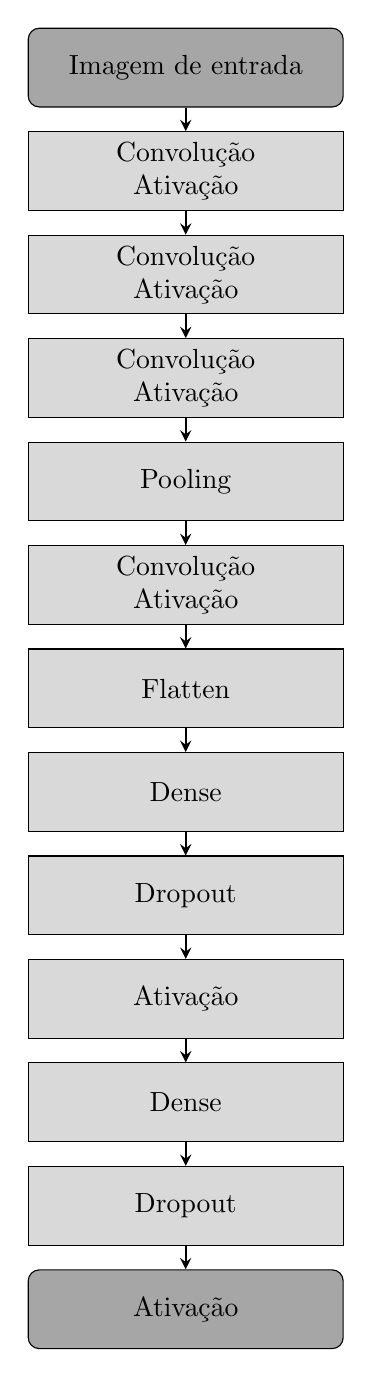
\begin{tikzpicture}[
	start chain=going below,
	every join/.style={arrow},
	node distance=0.3cm
	]
	\node (start) [startstop,on chain,join] {Imagem de entrada};
	
	\node (out1) [process,on chain,join] {Convolução \\ Ativação};
	
	\node (out3) [process,on chain,join] {Convolução \\ Ativação };
	
	\node (out5) [process,on chain,join] {Convolução \\ Ativação};
	
	\node (out7) [process,on chain,join] {Pooling};
	
	\node (out8) [process,on chain,join] {Convolução \\ Ativação};
	
	\node (out10) [process,on chain,join] {Flatten};
	\node (out11) [process,on chain,join] {Dense};
	
	\node (out12) [process,on chain,join] {Dropout};
	\node (out13) [process,on chain,join] {Ativação};	
	
	\node (out14) [process,on chain,join] {Dense};
	\node (out15) [process,on chain,join] {Dropout};
	
	\node (out16) [startstop,on chain,join] {Ativação};		
	
	\end{tikzpicture}%
	} %resizebox
	\caption{Arquitetura da rede CNN utilizada neste trabalho.}
		\label{tikz:mnist_cnn16}
\end{figure}

\par A implementação da rede descrita pela imagem \ref{tikz:mnist_cnn16} é exibida no código abaixo:
\begin{lstlisting}
from keras.layers import Activation
from keras.layers.convolutional import Convolution2D, MaxPooling2D
from keras.layers import Flatten, Dense
from keras.layers.core import Dropout

dropout_rate=0.3

modelo = Sequential()

def keras_add(m,op):
	m.add(op)
	l = m.layers[-1]

keras_add(modelo,Convolution2D(32, 2, 2,
	border_mode='valid', input_shape=(28, 28, 1)))
keras_add(modelo,Activation('relu'))

keras_add(modelo,Convolution2D(8, 12, 12))
keras_add(modelo,Activation('relu'))

keras_add(modelo,Convolution2D(16, 8, 8))
keras_add(modelo,Activation('relu'))

keras_add(modelo,MaxPooling2D(pool_size=(2, 2)))

keras_add(modelo,Convolution2D(32, 2, 2))
keras_add(modelo,Activation('relu'))

keras_add(modelo,Flatten())
keras_add(modelo,Dense(100))
keras_add(modelo,Dropout(dropout_rate))
keras_add(modelo,Activation('relu'))

keras_add(modelo,Dense(numero_classes))
keras_add(modelo,Dropout(dropout_rate))
keras_add(modelo,Activation('softmax'))
\end{lstlisting}

\par O objetivo das camadas convolucionais com ativação no início dessa rede é de encontrar características dos números e reduzir parcialmente o tamanho da imagem inicial antes do primeiro \textit{pooling}. Para melhor compreensão dos efeitos da convolução nas imagens foram utilizados em cada camada convolucional filtros dos tamanhos: 32 filtros de 2x2, 8 filtros de 12x12, 16 filtros de 8x8 e 32 filtros de 2x2.

\par A visualização dos filtros obtidos após o treinamento foi obtida da seguinte forma:

\begin{lstlisting}
img = np.zeros((28,28))
for a in xrange(28):
  for b in xrange(28):
    img[a][b] = X_treino[0][a,b]
    for i in xrange(len(modelo.layers)):
      m0 = modelo.layers[i]
      name = m0.name
      if "convolution" not in name:
        continue    
      ws = m0.get_weights()

      flt = np.zeros((np.shape(ws[0])[0],np.shape(ws[0])[1]))
      fig=plt.figure(figsize=(8,8))
      for oz in xrange(np.shape(ws[0])[2]):
        for z in xrange(np.shape(ws[0])[3]):
          ax = fig.add_subplot(6, 6, z+1)
          sa = np.shape(ws[0])[0]
          sb = np.shape(ws[0])[1]
          for a in xrange(sa):
            for b in xrange(sb):
              flt[a][b] = ws[0][a,b,oz,z]
              plt.xticks(np.array([]))
              plt.yticks(np.array([]))
              plt.tight_layout()        
              ax.imshow(flt,interpolation='nearest', cmap=plt.cm.gray) 
\end{lstlisting}


\par Os filtros descritos acima são visualizados na imagem \autoref{fig:convs_filtros}.

\begin{figure}[H]
	\centering
	
	\begin{subfigure}{.8\textwidth}
		\centering
		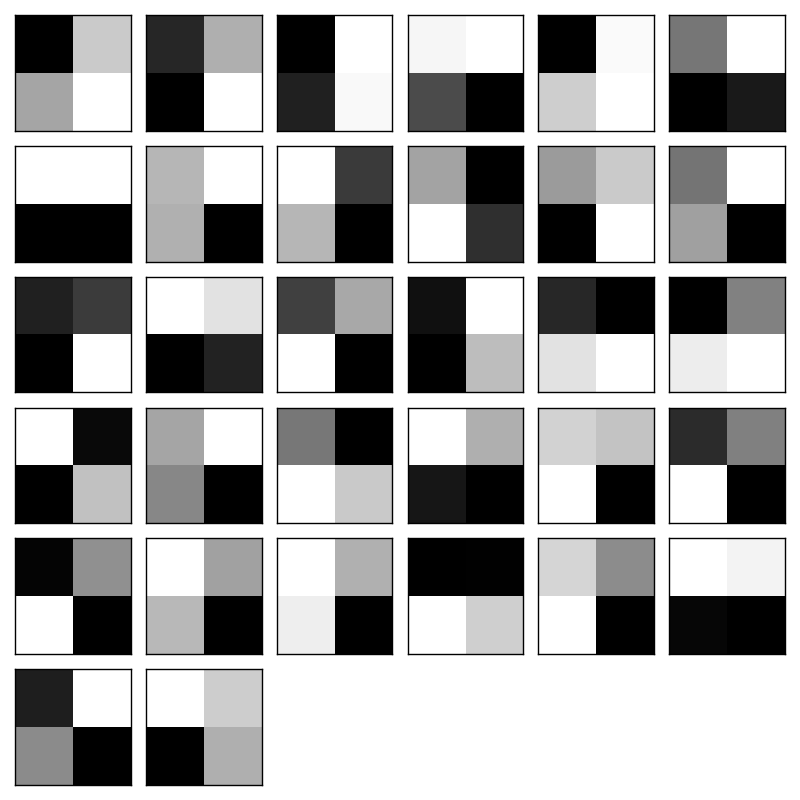
\includegraphics[width=.6\linewidth]{images/fabio/resultados/network_3/filter_convolution2d_1}%
		\caption{Filtros 2x2 - primeira convolução}		
		\label{fig:conv1_filtro}	
	\end{subfigure}%
	
	\begin{subfigure}{.8\textwidth}
		\centering
		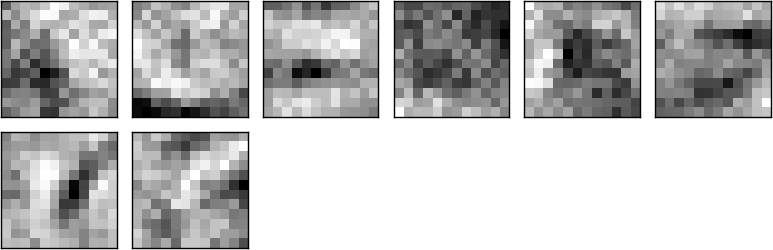
\includegraphics[width=.6\linewidth]{images/fabio/resultados/network_3/filter_convolution2d_2}
		\caption{Filtros 12x12 - segunda convolução}		
		\label{fig:conv2_filtro}	
	\end{subfigure}%
	
	\begin{subfigure}{.8\textwidth}
		\centering
		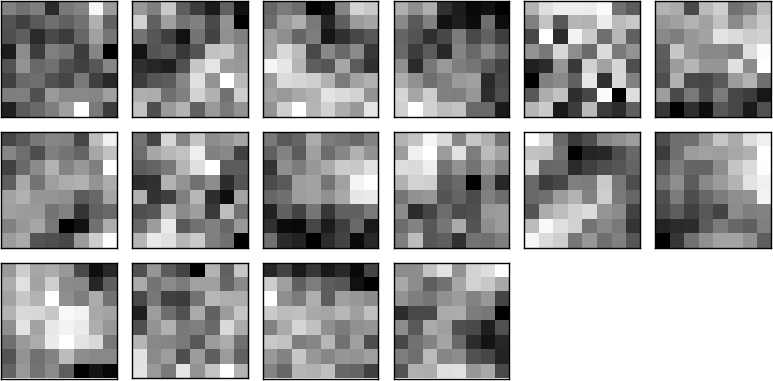
\includegraphics[width=.6\linewidth]{images/fabio/resultados/network_3/filter_convolution2d_3}%
		\caption{Filtros 8x8 - terceira convolução}		
		\label{fig:conv3_filtro}	
	\end{subfigure}%
d
	\begin{subfigure}{.8\textwidth}
	\centering
	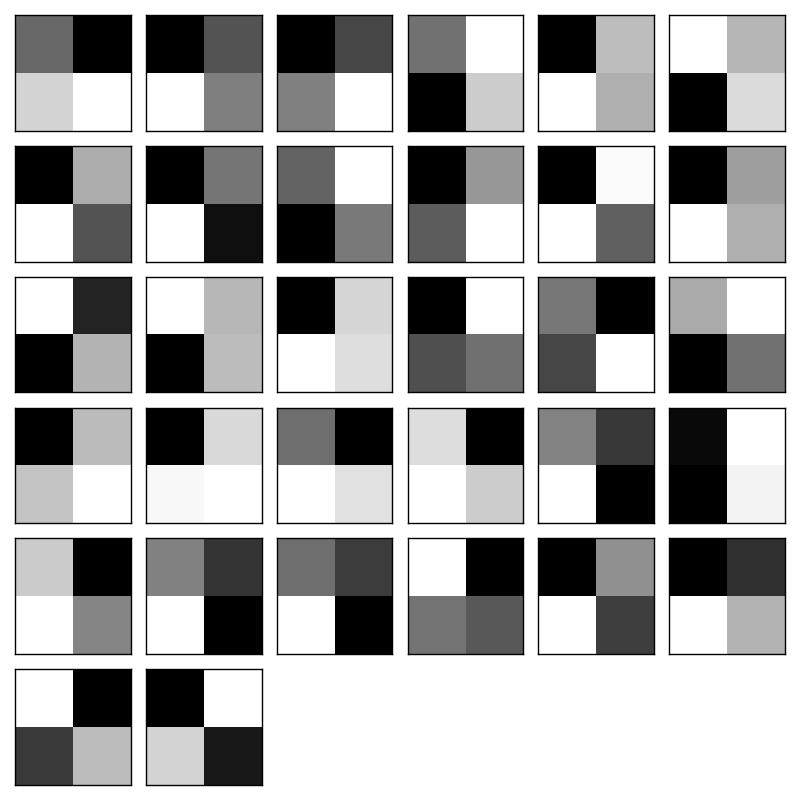
\includegraphics[width=.6\linewidth]{images/fabio/resultados/network_3/filter_convolution2d_4}%
	\caption{Filtros 2x2 - terceira convolução}		
	\label{fig:conv4_filtro}	
\end{subfigure}%
	\caption{Filtros convolucionais obtidos do treinamento.}
		\label{fig:convs_filtros}
\end{figure}


\par Após as primeiras camadas de convolução foi adicionada uma camada de \textit{pooling} para auxiliar na eliminação de ruídos e reduzir o número de elementos a serem explorados pela rede.
\par A seguir, uma nova camada de convolução foi adicionada para detectar novas características novamente. Por conta da estrutura do \textit{framework} do Keras, utilizado neste trabalho é necessário antes da rede \textit{fully-connected} ou (\textit{dense}) transformar a entrada em um vetor unidimensional, representada mais a frente por uma fita.
\par A camada \textit{dense} trabalha como uma camada de redes neurais conectando todos os elementos da entrada com todos os elementos da saída, visando estabelecer a relação da importância entre os elementos ativados e os resultados obtidos.
\par O próximo elemento é uma camada de \textit{Dropout} com objetivo de minimizar a dependência de algumas características específicas dos dígitos. Em seguida é utilizada uma camada de ativação para evidenciar os elementos mais importantes encontrados após a camada \textit{dense+droupout}.
\par Os últimos dois passos são novamente uma camada \textit{dense}, agora reduzindo as entradas de 100 para 10 elementos  (correspondentes aos dígitos de 0 a 9) e uma nova camada de ativação agora com função \textit{softmax} para ativação de um único elemento (representando a escolha da rede do elemento mais provável identificado pela rede).

\par A identificação do dígito é iniciada com a introdução da imagem contendo o item a ser identificado. Neste exemplo será utilizado o número 0 apresentado na imagem \ref{fig:numero_0}.

\begin{center}
\begin{figure}[H]
	\centering
	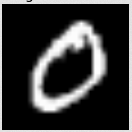
\includegraphics[width=0.3\linewidth]{images/fabio/numero_0}
	\caption{Número 0 escrito a mão disponível na base de dados do MNIST.}
	\label{fig:numero_0}
\end{figure}
\end{center}


\par A aplicação do primeiro conjunto de camada convolucional e ativação é mostrada em \autoref{fig:camada_1}. Apesar da aplicação dos filtros não resultar necessariamente em uma imagem humanamente compreensível é possível notar na ativação da \ref{fig:camada_1} que as bordas ficam ressaltadas em relação ao fundo e algumas das camadas buscam encontrar formatos específicos como linhas horizontais e verticais enquanto outras buscam formatos de curvas. 

\begin{center}
\begin{figure}[H]
\centering
\begin{subfigure}{.8\textwidth}
\centering
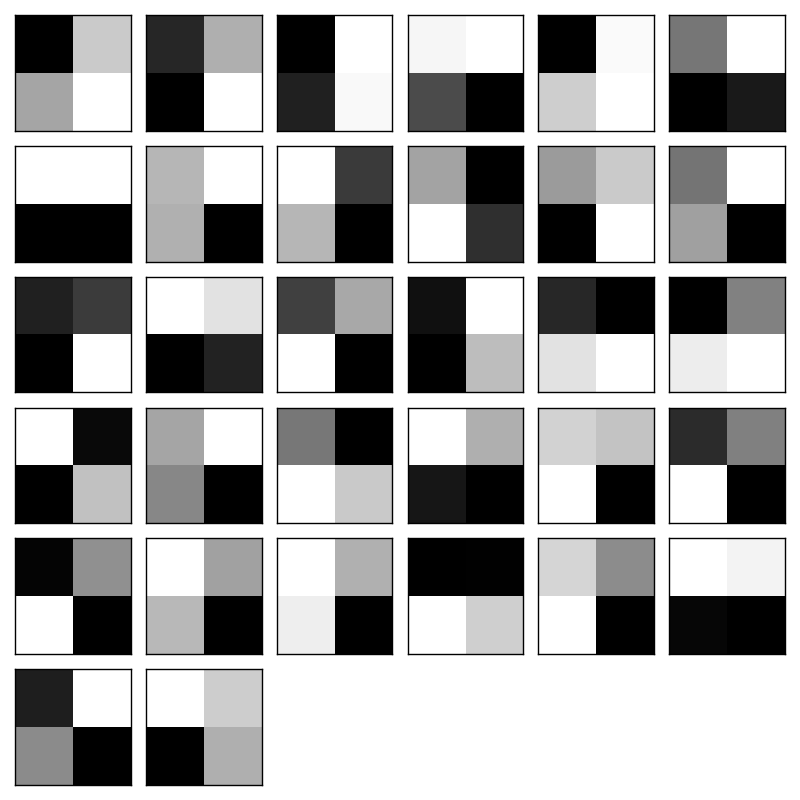
\includegraphics[width=.6\linewidth]{images/fabio/resultados/network_3/filter_convolution2d_1}%
\caption{Filtros 2x2 aplicados a primeira camada de convolução}		
\label{fig:filtros2x2}	
\end{subfigure}%

\begin{subfigure}{.8\textwidth}
\centering
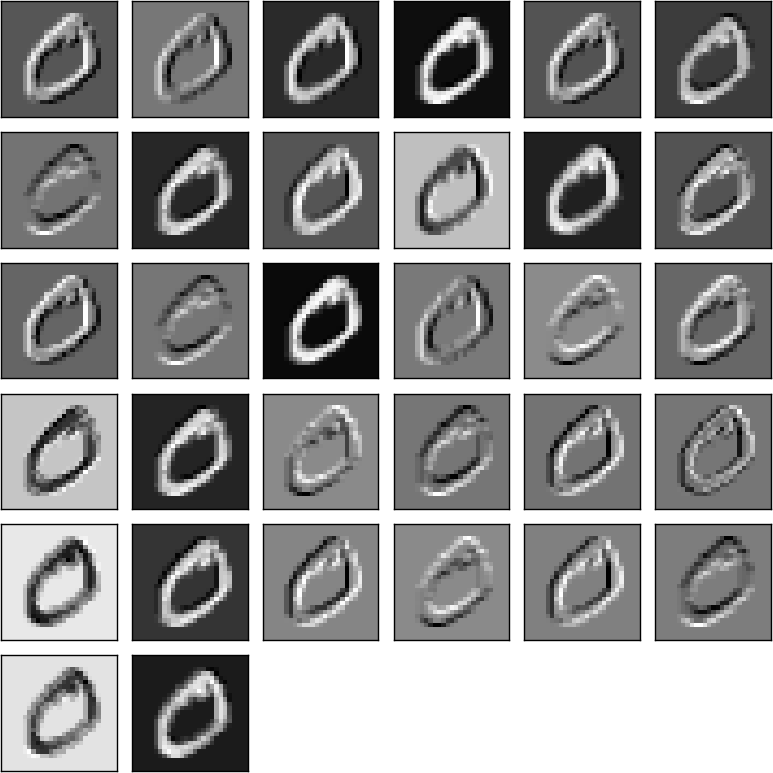
\includegraphics[width=.6\linewidth]{images/fabio/resultados/network_3/input_1_layer_convolution2d_1}
\caption{Convolução 1}
\end{subfigure}%

\begin{subfigure}{.8\textwidth}
\centering
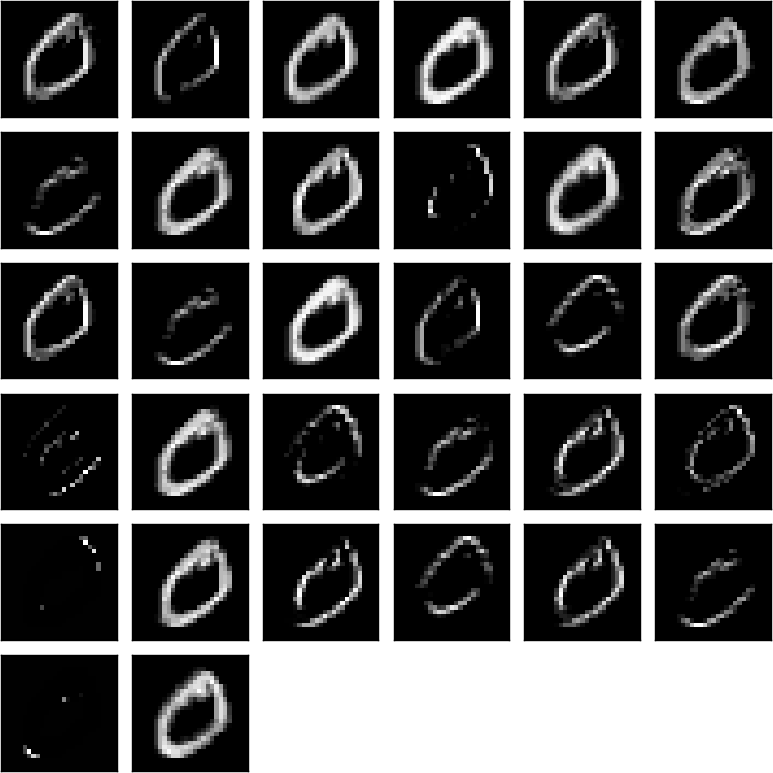
\includegraphics[width=.6\linewidth]{images/fabio/resultados/network_3/input_1_layer_activation_1}%
\caption{Ativação}			
\end{subfigure}%
\caption{Primeiro resultado da identificação no primeiro par de camadas de convolução e ativação.}
\label{fig:camada_1}
\end{figure}
\end{center}

%%%%%%%%%%%%%%%%%%%%%%%%%%%%%%%%%%%%%%%%%%%%%%%%%%%

\par Na segunda camada um filtro de tamanho 12x12 é utilizado. Novamente, apesar de não necessariamente ser uma imagem compreensível para humanos é possível notar no próprio filtro que alguns formtados de curvas e traços ficam evidenciado, indicando que esses filtros irão se ativar mais para esse tipo de padrão. O resultado na \autoref{fig:camada_2} tem a resolução menor por conta da redução no tamanho da saída. A saída dessa segunda camada é composta por varios componentes do número zero como bordas internas e externas além da evidenciação do centro do zero.

\begin{center}
\begin{figure}[H]
\begin{subfigure}{.8\textwidth}
	\centering
	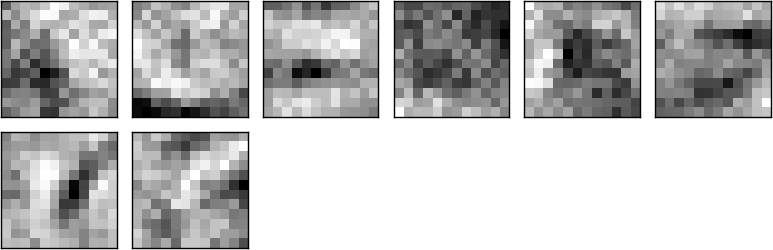
\includegraphics[width=.6\linewidth]{images/fabio/resultados/network_3/filter_convolution2d_2}%
	\caption{Filtros 12x12 aplicados a segunda camada de convolução}		
	\label{fig:filtros12x12}	
\end{subfigure}%

\begin{subfigure}{.8\textwidth}
	\centering
	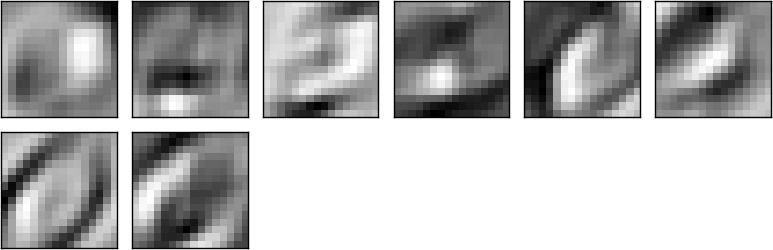
\includegraphics[width=.6\linewidth]{images/fabio/resultados/network_3/input_1_layer_convolution2d_2}
	\caption{Convolução 2}
\end{subfigure}%

\begin{subfigure}{.8\textwidth}
	\centering
	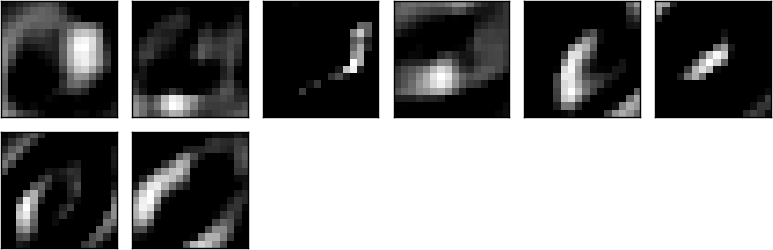
\includegraphics[width=.6\linewidth]{images/fabio/resultados/network_3/input_1_layer_activation_2}%
	\caption{Ativação}			
\end{subfigure}%
\caption{Primeiro resultado da identificação no segundo par de camadas de convolução e ativação.}
\label{fig:camada_2}
\end{figure}
\end{center}
%%%%%%%%%%%%%%%%%%%%%%%%%%%%%%%%%%%%%%%%%%%%%%%%%%%

\par A terceira camada utiliza um filtro 8x8, dessa vez praticamente nenhum elemento dos filtros é humanamente compreensível. A convolução nesta camada mostra que aguns filtros buscam por um padrão onde as bordas são preenchidas e o entro é vazio, e alguns outros filtros que também são mais ativados evidenciam o formato circular que o número zero tem.
\begin{center}
\begin{figure}[H]
	\begin{subfigure}{.8\textwidth}
		\centering
		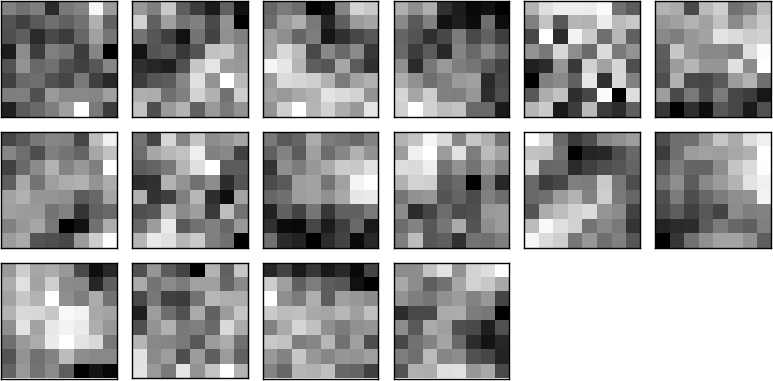
\includegraphics[width=.6\linewidth]{images/fabio/resultados/network_3/filter_convolution2d_3}%
		\caption{Filtros 8x8 aplicados a terceira camada de convolução}		
		\label{fig:filtros8x8}	
	\end{subfigure}%
	
	\begin{subfigure}{.8\textwidth}
		\centering
		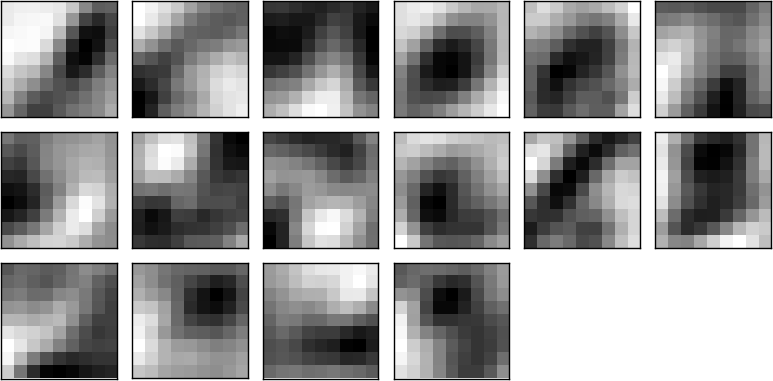
\includegraphics[width=.6\linewidth]{images/fabio/resultados/network_3/input_1_layer_convolution2d_3}
		\caption{Convolução 3}
	\end{subfigure}%
	
	\begin{subfigure}{.8\textwidth}
		\centering
		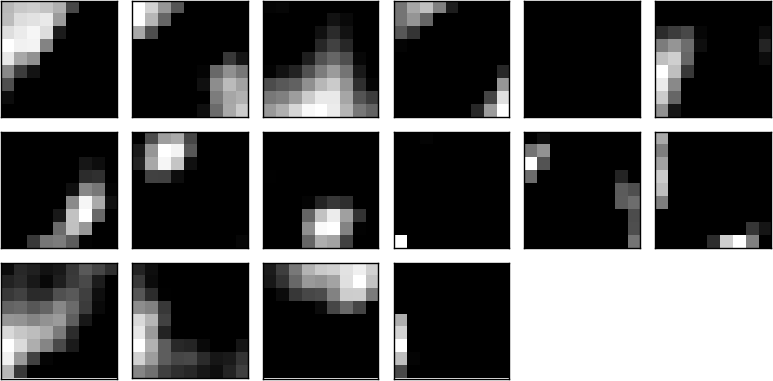
\includegraphics[width=.6\linewidth]{images/fabio/resultados/network_3/input_1_layer_activation_3}%
		\caption{Ativação}			
	\end{subfigure}%
	\caption{Primeiro resultado da identificação no terceiro par de camadas de convolução e ativação.}
		\label{fig:camada_3}
\end{figure}
\end{center}
%%%%%%%%%%%%%%%%%%%%%%%%%%%%%
\par A camada de \textit{pooling} tem como objetivo reduzir a dimensionalidade como é visto na \autoref{fig:input1layermaxpooling2d1}. O resultado da imagem com alguns dos filtro não possuem nenhum valor (filtro 5/16)=, enquanto outros capturam mais os pares de bordas (filtros 1/16 e 2/16) e outros apenas algumas bordas (filtros 14/16 e 15/16).

\begin{center}
\begin{figure}[H]
	\centering
	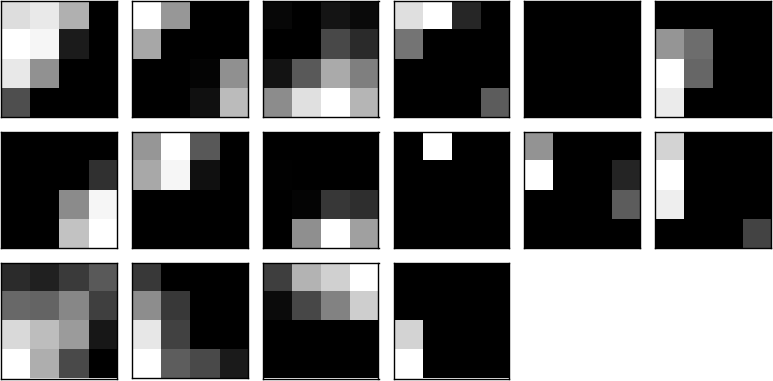
\includegraphics[width=0.5\textwidth]{images/fabio/resultados/network_3/input_1_layer_maxpooling2d_1}
	\caption{Resultado da camada de Pooling}
	\label{fig:input1layermaxpooling2d1}
\end{figure}
\end{center}

%%%%%%%%%%%%%%%%%%%%%%%%%%%%%%%%%%%%%%%%%%%%%%%%%%%
\par Na quarta camada de convolução o resultado é uma imagem de 3x3 pixels. Não é possível afirmar exatamente o que cada resultado representa (por conta da forma como o aprendizado de máquina funciona), mas é possível verificar que o ponto mais ativo em cada filtro  representa uma relação dentre cada um dos 9 pixels da imagem e os elementos adjacentes.

\begin{center}
\begin{figure}[H]
	\begin{subfigure}{.8\textwidth}
		\centering
		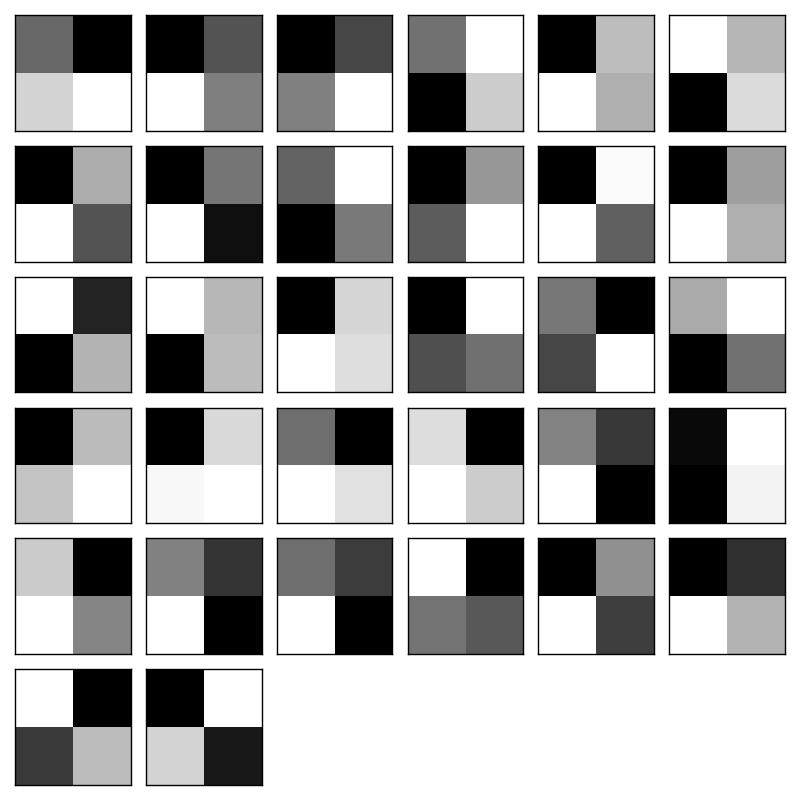
\includegraphics[width=.6\linewidth]{images/fabio/resultados/network_3/filter_convolution2d_4}%
		\caption{Filtros 2x2 aplicados a quarta camada de convolução}		
		\label{fig:filtros2x2_4}	
	\end{subfigure}%
	
	\begin{subfigure}{.8\textwidth}
		\centering
		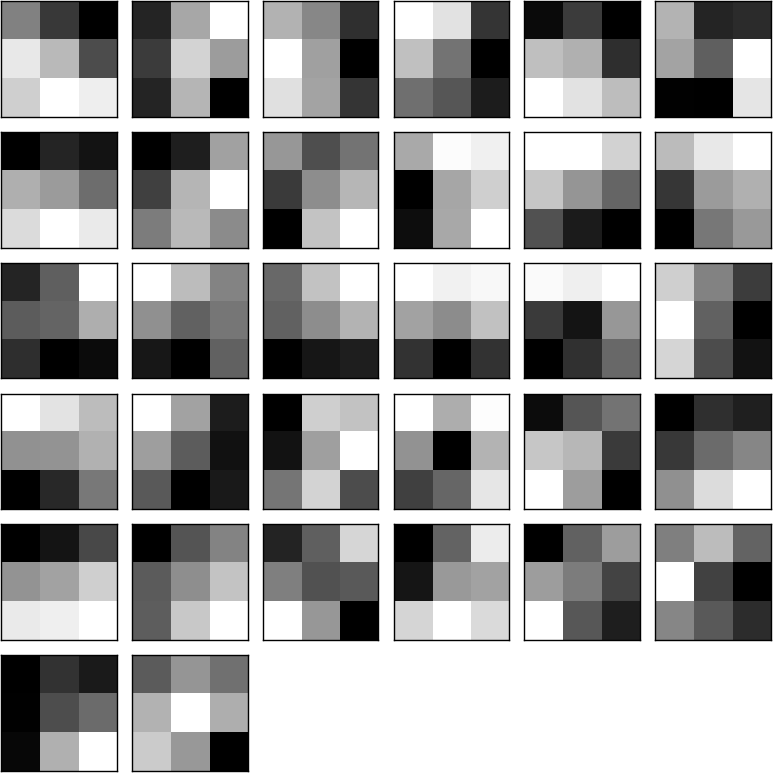
\includegraphics[width=.6\linewidth]{images/fabio/resultados/network_3/input_1_layer_convolution2d_4}
		\caption{Convolução 4}
	\end{subfigure}%
	
	\begin{subfigure}{.8\textwidth}
		\centering
		
\includegraphics[width=.6\linewidth]{images/fabio/resultados/network_3/input_1_layer_activation_4}%
		\caption{Ativação}			
	\end{subfigure}%
	\caption{Primeiro resultado da identificação no quarto par de camadas de convolução e ativação.}
		\label{fig:camada_2}
\end{figure}
\end{center}
%%%%%%%%%%%%%%%%%%%%%%%%%%%%%%%%%%%%%
\par A função Flatten do Keras, \autoref{fig:input1flatten}, transformar um item multidimensional em um vetor unidimensional. Neste caso 3x3x32 (imagem 3x3 e 32 filtros) transformasse em um vetor 1x1x288. Este artifício é utilizado para pode realizar a interface com a camada de treinamento \textit{fully connected} (totalmente conectada) assim como no aprendizado clássico de redes neurais.
\begin{center}
\begin{figure}[H]
	\centering
	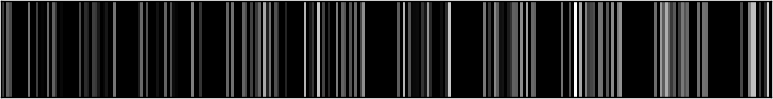
\includegraphics[width=0.5\textwidth]{images/fabio/resultados/network_3/input_1_layer_flatten_1}
	\caption{Resultado da camada de Flatten}
	\label{fig:input1flatten}
\end{figure}
\end{center}

%%%%%%%%%%%%%%%%%%%%%%%%%%%%%%%%%%%%%
\par A camada Dense do Keras, \autoref{fig:input1dense1}, representa o treinamento clássico de redes neurais onde cada elemento da entrada é ligado a todos os elementos da camada escondida que por sua vez é ligado por todos os elementos de saída. Como as camadas anteriores reduziram a dimensionalidade da imagem o treinamento nesta fase é relativamente rápido por contar com 288 elementos de entrada e 100 elementos de saída apenas.
\begin{center}
\begin{figure}[H]
	\centering
	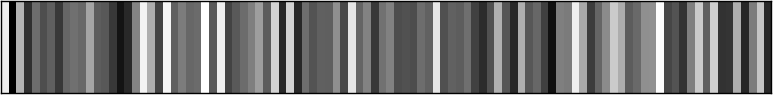
\includegraphics[width=0.5\textwidth]{images/fabio/resultados/network_3/input_1_layer_dense_1}
	\caption{Resultado da camada Dense}
	\label{fig:input1dense1}
\end{figure}
\end{center}


%%%%%%%%%%%%%%%%%%%%%%%%%%%%%%%%%%%%%
\par Uma camada de ativação é adicionada em \autoref{fig:input1atv5} com objetivo de passar para a próxima camada apenas os elementos mais importantes e eliminar possíveis ruídos no treinamento.
\begin{center}
\begin{figure}[H]
	\centering
	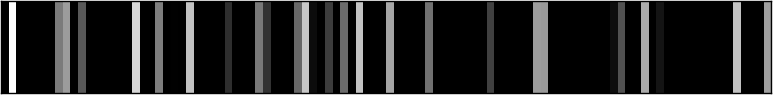
\includegraphics[width=0.5\textwidth]{images/fabio/resultados/network_1/input_1_layer_activation_7}
	\caption{Resultado da camada de ativação antes da saída}
	\label{fig:input1atv5}
\end{figure}
\end{center}
%%%%%%%%%%%%%%%%%%%%%%%%%%%%%%%%%%%%%
\par Uma nova camada Dense é adiciona agora para realizar a classificação entre 10 itens (número de 0 a 9).
\begin{center}
\begin{figure}[H]
	\centering
	
\includegraphics[width=0.5\textwidth]{images/fabio/resultados/network_1/input_1_layer_dense_2}
	\caption{Resultado da camada de ativação antes da saída}
	\label{fig:input1dense2}
\end{figure}
\end{center}
%%%%%%%%%%%%%%%%%%%%%%%%%%%%%%%%%%%%%
\par A ultima camada de ativação elimina os outros resultados menos prováveis e mantém apenas o elemento que foi mais ativado. Neste caso apenas o único elemento do vetor com indice zero representando o número 0.
\begin{center}
\begin{figure}[H]
	\centering
	
\includegraphics[width=0.5\textwidth]{images/fabio/resultados/network_1/input_1_layer_activation_8}
	\caption{Resultado da camada de ativação para definição da saída}
	\label{fig:input1atv7}
\end{figure}
\end{center}
% ---
% Conclusão
% ---
\chapter{Conclusão}
% ---

\par O resultado da arquitetura apresentada na seção anterior foi de 98.89\% para os elementos de treino da base do MNIST e de 99.06\% para os elementos de teste da mesma base. Tais resultados demonstram que a aplicação da técnica de redes convolucionais para este problema foi efetiva se comparando a outros bons resultados demonstrados em outras redes convolucionais em \citeonline{mnistlecunn}.



% ----------------------------------------------------------
% ELEMENTOS PÓS-TEXTUAIS
% ----------------------------------------------------------
%\postextual

% ----------------------------------------------------------
% Referências bibliográficas
% ----------------------------------------------------------
\bibliography{bibliografia}

% ----------------------------------------------------------
% Glossário
% ----------------------------------------------------------
%
% Consulte o manual da classe abntex2 para orientações sobre o glossário.
%
%\glossary

% ----------------------------------------------------------
% Apêndices
% ----------------------------------------------------------

% ---
% Inicia os apêndices
% ---
%\begin{apendicesenv}

% Imprime uma página indicando o início dos apêndices
%\partapendices

% ----------------------------------------------------------
%\chapter{Quisque libero justo}
% ----------------------------------------------------------

%\lipsum[50]

% ----------------------------------------------------------
%\chapter{Nullam elementum urna vel imperdiet sodales elit ipsum pharetra ligula
%ac pretium ante justo a nulla curabitur tristique arcu eu metus}
%% ----------------------------------------------------------
%\lipsum[55-57]
%
%\end{apendicesenv}
%% ---
%
%
%% ----------------------------------------------------------
%% Anexos
%% ----------------------------------------------------------
%
%% ---
%% Inicia os anexos
%% ---
%\begin{anexosenv}
%
%% Imprime uma página indicando o início dos anexos
%\partanexos
%
%% ---
%\chapter{Morbi ultrices rutrum lorem.}
%% ---
%\lipsum[30]
%
%% ---
%\chapter{Cras non urna sed feugiat cum sociis natoque penatibus et magnis dis
%parturient montes nascetur ridiculus mus}
%% ---
%
%\lipsum[31]
%
%% ---
%\chapter{Fusce facilisis lacinia dui}
%% ---
%
%\lipsum[32]
%
%\end{anexosenv}
%
%%---------------------------------------------------------------------
%% INDICE REMISSIVO
%%---------------------------------------------------------------------
%
%\phantompart
%
%\printindex
%
%%---------------------------------------------------------------------
%% Formulário de Identificação (opcional)
%%---------------------------------------------------------------------
%\chapter*[Formulário de Identificação]{Formulário de Identificação}
%\addcontentsline{toc}{chapter}{Exemplo de Formulário de Identificação}
%\label{formulado-identificacao}
%
%Exemplo de Formulário de Identificação, compatível com o Anexo A (informativo)
%da ABNT NBR 10719:2015. Este formulário não é um anexo. Conforme definido na
%norma, ele é o último elemento pós-textual e opcional do relatório.
%
%\bigskip
%
%\begin{tabular}{|p{9cm}|p{5cm}|}
%\hline
%\multicolumn{2}{|c|}{\textbf{\large Dados do Relatório Técnico e/ou científico}}\\
%\hline
%\multirow{4}{10cm}[24pt]{Título e subtítulo}& Classificação de segurança\\
%                   & \\
%                   \cline{2-2}
%                   & No.\\
%                   & \\
%				
%\hline
%Tipo de relatório & Data\\
%\hline
%Título do projeto/programa/plano & No.\\
%\hline
%\multicolumn{2}{|l|}{Autor(es)} \\
%\hline
%\multicolumn{2}{|l|}{Instituição executora e endereço completo} \\
%\hline
%\multicolumn{2}{|l|}{Instituição patrocinadora e endereço completo} \\
%\hline
%\multicolumn{2}{|l|}{Resumo}\\[3cm]
%\hline
%\multicolumn{2}{|l|}{Palavras-chave/descritores}\\
%\hline
%\multicolumn{2}{|l|}{
%Edição \hfill No. de páginas \hfill No. do volume \hfill Nº de classificação \phantom{XXXX}} \\
%\hline
%\multicolumn{2}{|l|}{
%ISSN \hfill \hfill Tiragem \hfill Preço \phantom{XXXXXXXX}} \\
%\hline
%\multicolumn{2}{|l|}{Distribuidor} \\
%\hline
%\multicolumn{2}{|l|}{Observações/notas}\\[3cm]
%\hline
%\end{tabular}

\end{document}
